\section{Implementation Development Plan}

In all the steps of implementation, there will be 2 entities that will need to communicate with each other through the Lightning Network. The entities will be called A and B.

For all the steps the aim will be to ensure that the two entities, A and B, can communicate in the correct way. The two activity diagrams shown below in figure \ref{fig:activity_diagrams} outline the scenarios that should be tested at each step in the development. The activity diagram in figure \ref{fig:test_1} shows the most basic form of transaction that should happen between entity A and B in which B will produce an invoice that A will then pay. The activity diagram shown in figure \ref{fig:test_2} shows a more complicated scenario where after having established an initial connection, entity A can continue to use a resource provided by B and be charged for the resource in micropayments.

\begin{figure}[h!]
     \centering
     \begin{subfigure}[b]{0.2\textwidth}
         \centering
         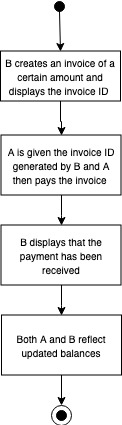
\includegraphics[width=\textwidth]{activity_1.jpg}
         \caption{Test 1}
         \label{fig:test_1}
     \end{subfigure}
     \hfill
     \begin{subfigure}[b]{0.4\textwidth}
         \centering
         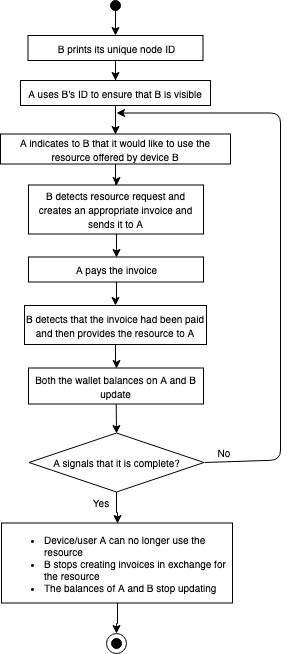
\includegraphics[width=\textwidth]{activity_2.jpg}
         \caption{Test 2}
         \label{fig:test_2}
     \end{subfigure}
     \caption{Activity diagrams showing implementation tests}
      \label{fig:activity_diagrams}
\end{figure}

\subsection{Step 1}

\begin{enumerate}[label=\alph*)]
    \item Download the Bitcoin blockchain onto a laptop computer
    \item Install and set up a Bitcoin server (bitcoind) and a Lightning Server (lnd)
    \item Create two separate Lightning wallets and instances so that it is as if two different devices on the Lightning Network exist.
    \item  Implement and test two programs that recreate the scenarios shown in the activity diagrams in figure \ref{fig:activity_diagrams}.
\end{enumerate}

\begin{figure}[h!]
\centering
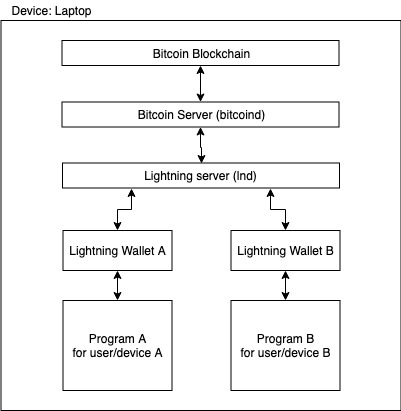
\includegraphics[scale=0.5]{Figures/step1.jpg}
\caption{Step 1 block diagram}
\label{fig:step1}
\end{figure}


\subsection{Step 2}

\begin{enumerate}[label=\alph*)]
    \item Set up Bitcoin and Lightning on a Raspberry Pi device
    \item Implement and test two programs that recreate the scenarios shown in the activity diagrams in figure \ref{fig:activity_diagrams}. (This will require manually informing device A of the Lightning node ID of device B.
\end{enumerate}

\begin{figure}[h!]
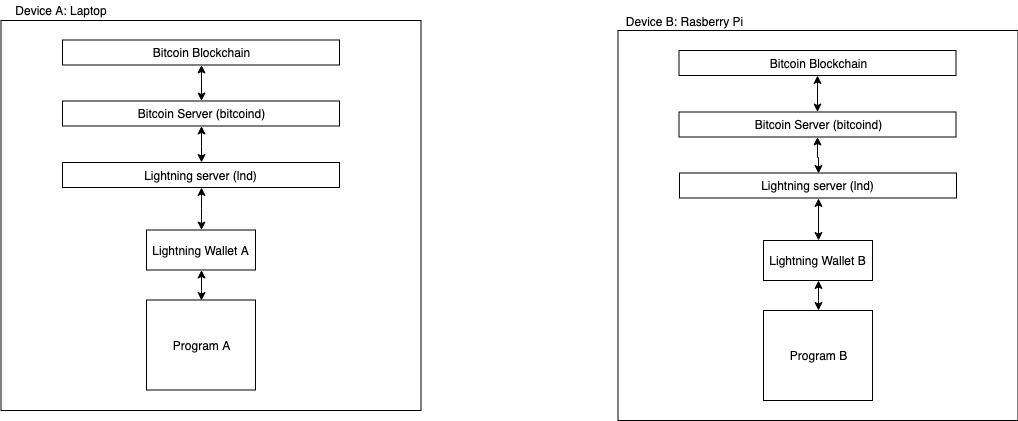
\includegraphics[scale=0.5]{Figures/step2.jpg}
\caption{Step 2 block diagram}
\label{fig:step2}
\end{figure}

\subsection{Step 3}

\begin{enumerate}[label=\alph*)]
    \item Integrate a camera and QR reader into system A
    \item Integrate a display and QR presenter into system B
    \item Implement and test two programs that recreate the scenarios shown in the activity diagrams in figure \ref{fig:activity_diagrams} but with the following developments:
        \begin{itemize}
            \item B displays its invoice/ID info on the QR display
            \item A gets B’s invoice/ID data from its camera and QR decoder
        \end{itemize}
\end{enumerate}

\begin{figure}[h!]
\centering
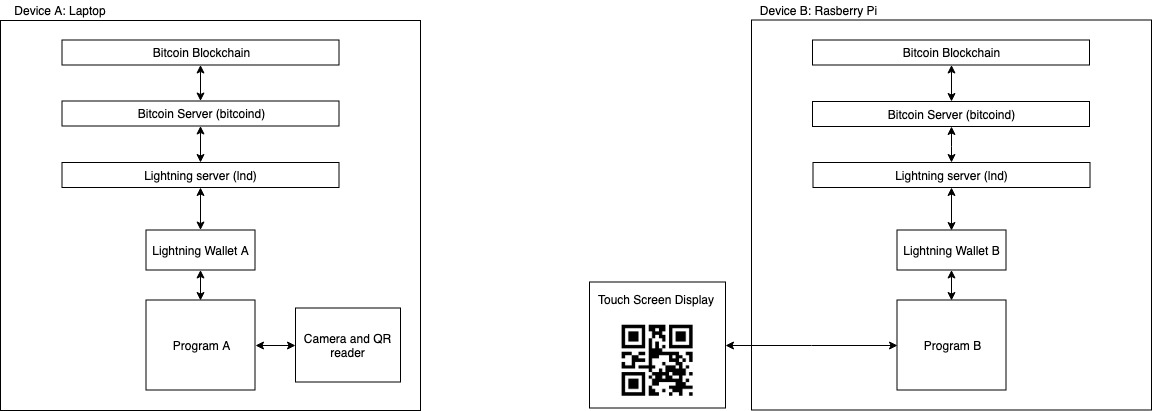
\includegraphics[scale=0.5]{Figures/step3.jpg}
\caption{Step 3 block diagram}
\label{fig:step3}
\end{figure}

\subsection{Step 4}

\begin{enumerate}[label=\alph*)]
    \item Add details such as a user interface for both A and B
    \item Add a potentiometer and configure its input to represent the amount of the resource that A is using and ensure that B creates invoices with amounts based on the potentiometer reading.
    \item Add an LED as a way for B to show that its resource is or is not currently available to A.
\end{enumerate}

\begin{figure}[h!]
\centering
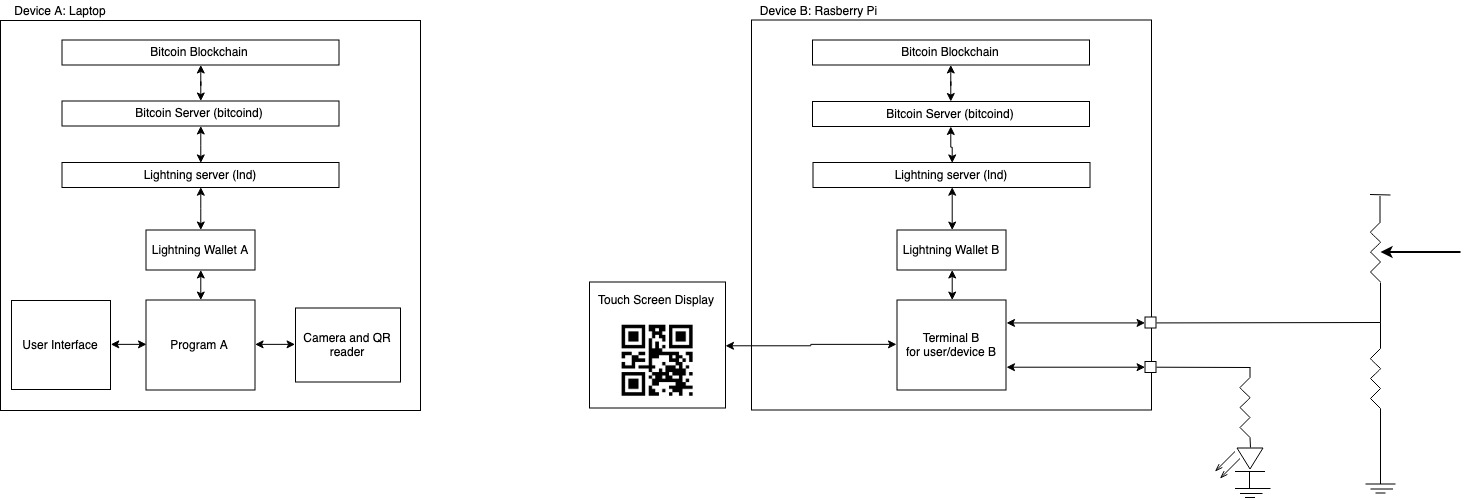
\includegraphics[scale=0.5]{Figures/step4.jpg}
\caption{Step 4 block diagram}
\label{fig:step4}
\end{figure}